\chapter{Prezentare turbine "AXENT"}\label{chapter:prezentare}


\section{Utilitate și utilizare}

\subsection{Introducere}

Datorită creșterii continue a consumului global de energie problemelor legate de creșterea emisiilor de gaze cu efect de seră ce duc la schimbări climatice, creșterea eficienței energetice este o nevoie speciala  și urgenta. Pe lângă implementarea de sisteme de producere a energiei regenerabile o soluție e reprezentata și de eficientizarea energetica a proceselor deja existente. În cadrul acestei lucrări este studiata eficientizarea unei turbine axiale de expansiune pentru a contribui la procesul de reducere a consumului de energie.


\subsection{Recuperarea energiei de la fluidele de lucru}

În multe procese industriale, fluidele de lucru se află la un nivel mai ridicat de presiune decât este necesar. În cele mai multe cazuri, este destinsa prin supape convenționale, energia potențiala de presiune rămânând astfel neutilizata. Prin recuperarea energiei sub presiune, eficiența globală a sistemelor respectiva este crescuta.

O modalitate de a recupera energia din fluidele de lucru este utilizarea unor mașini hidraulice. În multe procese se pot folosi turbine hidraulice sau PAT (Pump as turbine - pompe în regim de turbina) pentru transformarea pierderilor sub forma de căldura care se întâmpla prin supape în energie electrica ce poate fi redistribuita în sistem.


\subsubsection{Domenii de aplicare existente}

Pana în acest moment nu exista multe domenii în care se încearcă câștigarea energiei din fluidele de lucru sub presiune. Un domeniu în care exista aplicabilitate de câteva decenii este cel al alimentarii cu apa potabila. Alte domenii de aplicabilitate sunt cele de desalinizare și de epurare a gazului. Cu toate acestea, în acest moment, domeniul de aplicabilitate principal rămâne cel de recuperare a energiei din procesele de alimentare cu apa unde turbinele axiale și PAT-urile câștiga o popularitate tot mai mare ca înlocuitoare a supapelor de control a presiunii.

Conductele de apa potabila sunt de obicei dimensionate generos, rezistând și la momentele de încărcare maxima fără probleme. În zonele muntoase, zonele care au și cel mai mare potențial de utilizare, trebuie depășite anumite diferențe de altitudine intre zona de alimentare și zona de distribuție. Energia reziduala astfel apărută din presiunea mare existenta la distribuire putând fi recuperata.


\subsubsection{Aplicații potențiale}

În plus față de domeniile de aplicare deja existente menționate mai sus, există multe altele în care energia ar putea fi recuperată din lichide de lucru. Posibile domenii de aplicare se regăsesc, de exemplu, în industria petrolieră, chimică și industria petrochimică, industria celulozei și hârtiei, precum și în domeniul geotermal.


\subsection{Stadiul tehnicii}

În prezent se folosesc în majoritatea cazurilor de recuperare a energiei fluidelor de lucru pompe centrifuge folosite în regim de turbină. Acestea sunt ușor disponibile în comerț, iar acest mod de funcționare este denumit în literatura de specialitate ca "pump as turbine" sau PAT. În imagine Figura 1.1 este o reprezentare schematică a unei pompe centrifuge clasice.

\begin{figure}[h!]
	\centering
	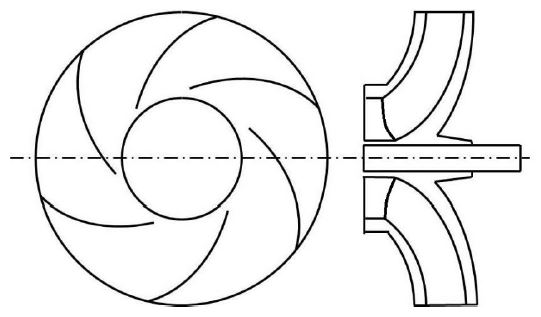
\includegraphics[scale=0.7]{figures/centrifugal-pump.jpg}
	\caption{Pompa centrifugă clasică \cite{neipp2017zweistufige}}
	\label{Pompa centrifugă clasică \u{a}}
\end{figure}

Cea mai mare provocare în recuperarea energiei de la fluidele de lucru nu este conversia în energie electrică, ci integrarea în sistemul respectiv, fără a pierde proprietățile sistemului și
Influența negativă asupra stabilității procesului.

La sfârșitul anilor '90, ideea unei turbine axiale de destindere, a apărut în calitate de concurent pentru pompele care funcționau în regim de turbine. Apoi a fost dezvoltata de Universitatea din Stuttgart, microturbina AXENT, optimizate din punct de vedere hidraulic.


\subsubsection{Compararea AXENT cu un PAT}

Figura 1.2 prezintă o comparație între curbele caracteristice a unei turbine AXENT și un PAT clasic. Pe baza curbei caracteristice devine clar că debitul în turbina AXENT rămâne aproape constant debitul chiar și la o variație puternica a numărului de rotații atinse de turbine în anumite situații critice.. În schimb, PAT prezintă un comportament complet diferit. Se poate observa că debitul scade brusc cu creșterea vitezei. Din cauza acestei proprietăți se așteaptă ca și în cazul unei deconectări de la rețea atunci când turația creste, presiunea nu scade cu o valoare mai mare de 10\%.

\begin{figure}[h!]
	\centering
	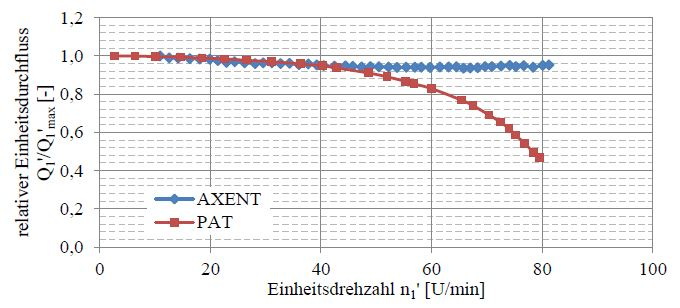
\includegraphics[scale=0.7]{figures/axent-pat.jpg}
	\caption{Comparația curbelor caracteristice AXENT și PAT \cite{neipp2017zweistufige}}
	\label{Comparația curbelor caracteristice AXENT și PAT\u{a}}
\end{figure}

În cazul PAT se integrează dispozitive de siguranță suplimentare și supapele de comandă sunt necesare, ceea ce sporește semnificativ cerința de spațiu a sistemului de recuperare a energiei. Îndeplinirea cerinței spațiale, asigurând în același timp siguranța instalațiilor și stabilitatea proceselor reprezintă principalele avantaje ale AXENT față de PAT-urile convenționale. Domeniile de aplicare ale AXENT sunt mult mai flexibile și gama posibilă de aplicare este mai mare.


\subsubsection{Proprietăți specifice turbinei AXENT}

Posibilele domenii de aplicare a turbinei AXENT, descrise în secțiunea 1.1.2 au în comun faptul ca în conducte avem o presiune mare cu debite mici astfel rezulta o turație specifica pentru acest tip de turbine relativ mica pentru o turbina axiala. Prin turația specifica \(n_q\) se descrie legătura teoretica dintre turație \(n\), căderea \(h\) și debitul prin turbina \(Q\) sub forma următoare:

\begin{equation}
n_q = n \cfrac{\sqrt{Q}}{H^\frac{3}{4}}
\end{equation}

Turațiile specifice mari pentru o turbina axiala, specifice turbinei AXENT duc la apariția unui număr mare de palete, mai degrabă asemănător turbinelor de gaz sau abur, numărul de profile crescând odată cu scăderea turației specifice. Fata de turbinele Kaplan sau Pelton, avem mult mai mult palete pe rotorul acestor turbine, în schimb acestea sunt fixe, neexistând posibilitatea ajustării unghiului acestora. În capitolele următoare este studiata în amănunt geometria acestor palete.

Condițiile tehnice asumate inițial au presupus găsirea de soluții unde avem:

\begin{itemize}
	\item fluid de lucru la presiune ridicat\u{a}
		\begin{itemize}
			\item transport
			\item procese industriale
		\end{itemize}
	\item destinderea presiunii p\^{a}n\u{a} la nivelul dorit
		\begin{itemize}
			\item făcută prin robineți, supape sau armaturi
			\item energia potențială a presiunii rămânând nefolosit\u{a}
		\end{itemize}
	\item creșterea randamentului prin recâștigarea de energie
		\begin{itemize}
			\item transformarea energiei hidraulice \^{i}n energie electric\u{a}
			\item far\u{a} a afecta instala\c{t}ia sau procesul deja existent
		\end{itemize}	
\end{itemize}

Pentru situa\c{t}iile enumerate mai sus dorința a fost de a îndeplini mai multe lucruri dintre care le voi enumera pe cele mai importante:

\begin{itemize}
	\item proprietăți tehnice
		\begin{itemize}
			\item utilizare la debit constant
			\item lipsa șocurilor hidraulice (a loviturii de berbec atunci când fluidul este frânat sau accelerat în timp foarte scurt, datorita închiderii rapide a vanelor și robinetelor)
			\item domeniu de utilizare larg
		\end{itemize}
	\item domenii potențiale de utilizare
		\begin{itemize}
			\item alimentare cu apă
			\item procese industriale
			\item industria chimică
		\end{itemize}
	\item din punct de vedere economic
		\begin{itemize}
			\item recuperare de energie
			\item costuri de realizare și întreținere cat mai mici
		\end{itemize}
	\item obiective politice
		\begin{itemize}
			\item eficientizare sistemelor și proceselor din diferite domenii ca dorința constanta (turbina AXENT nefiind o mașină primara de producere de energie, ci o metodă de eficientizare a procesului de alimentare cu apă)
			\item îmbunătățirea bilanțurilor ecologice
		\end{itemize}	
\end{itemize}

După analiza tuturor criteriilor pentru care se cauta o soluție, respectând bineînțeles și condițiile economice și politice, concluzia a fost ca cel mai bun loc pentru aceasta viitoare turbină este în domeniul \textbf{alimentarii cu apa a orașelor mari din zone muntoase}, o reprezentare schematica a acestei situații fiind vizibila în Figura 1.3.

\begin{figure}[h!]
	\centering
	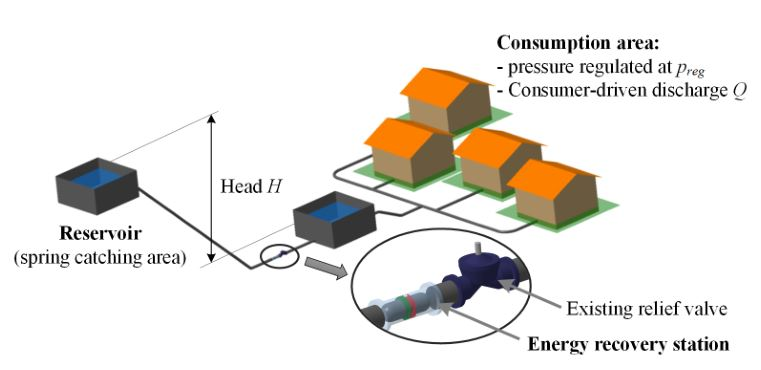
\includegraphics[scale=0.5]{figures/amplasare_turbina.jpg}
	\caption{Amplasare turbină \cite{andolfatto2016simulation}}
	\label{Amplasare turbin\u{a}}
\end{figure}

Condițiile minime care trebuie îndeplinite sunt legate de topografia regiunii, pentru a avea o cădere și o presiune mare, dar și mărimea rețelei de alimentare pentru a asigura debitul necesar funcționarii turbinei la randament ridicat. În principiu este necesara o topografie deluroasa și alimentarea cu apa sa se facă pentru o comunitate de minim 3000 de locuitori.


\section{Particularități constructive}

Turbinele de destindere au ca elemente principale un rotor, căruia datorita mișcării apei îi este imprimata o mișcare de rotație ai un generator pentru transformarea lucrului mecanic în energie electrica. Un punct după care putem categorisi turbinele axiale de destindere este poziția generatorului, varianta "Inline" (vezi Figura 1.4) cu generator imersat în conductă imediat după rotor sau cu generator aflat în afara conductei de trecere a apei, generator exterior (Figura 1.5).

\begin{figure}[h!]
	\centering
	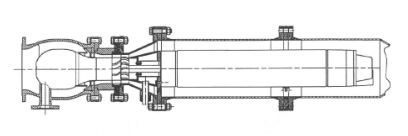
\includegraphics[scale=1]{figures/generator_inline.jpg}
	\caption{Generator imersat "Inline" \cite{GREES_2014}}
	\label{Generator imersat Inline}
\end{figure}

\begin{figure}[h!]
	\centering
	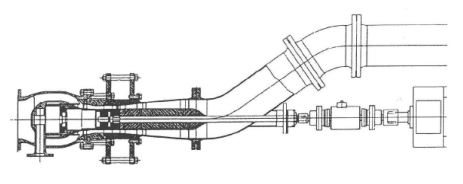
\includegraphics[scale=1]{figures/generator_in_afara_conductei.jpg}
	\caption{Generator în afara conductei \cite{GREES_2014}}
	\label{Generator în afara conductei}
\end{figure}

După cum se vede și în ultimele imagini, avantajul turbinei cu generator "Inline" constă în capacitatea de instalare modulara mult mai simpla, prin secționarea conductei și prinderea modulului turbinei prin flanșe în conductă.

În proiectarea moderna a turbinelor axiale, se folosește frecvent teoria hidrodinamică a rețelelor de profile. Metodele numerice de determinare a rețelelor de profile, care exprima legătura intre parametrii geometrici și cei hidrodinamici au fost folosite în cadrul Universității Suttgart pentru a ajunge la un produs cu aplicabilitate imediata și tangibila. Rezultatele acestor cercetări au fost dezvoltarea unei turbine cu aparat director format din 26 profile și un rotor cu 30 palete, care se poate folosi în modul singular sau în doua trepte (vezi Figura 1.6 și Figura 1.7).

\begin{figure}[h!]
	\centering
	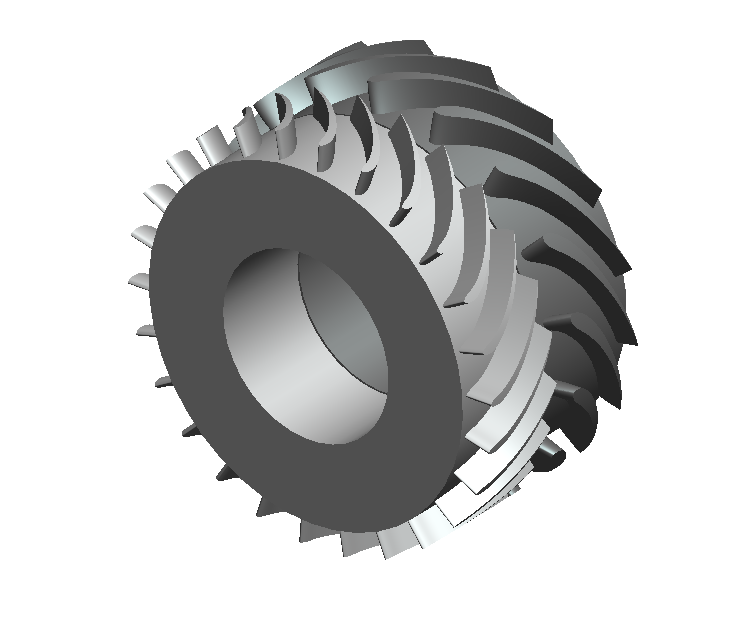
\includegraphics[scale=0.6]{figures/modul_singular.png}
	\caption{Modul singular \cite{susanhub}}
	\label{Modul singular}
\end{figure}

\begin{figure}[h!]
	\centering
	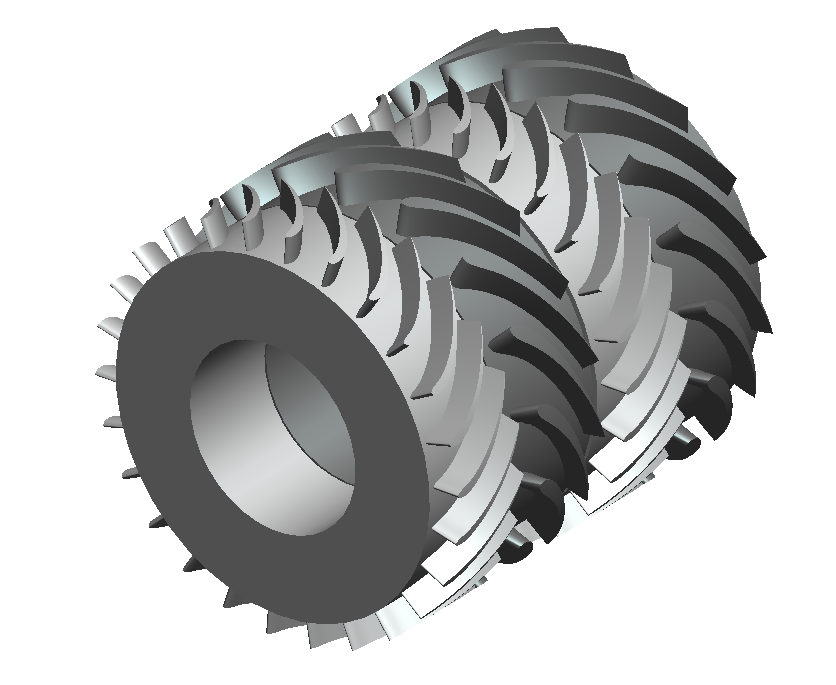
\includegraphics[scale=0.6]{figures/modul_in_doua_trepte.png}
	\caption{Modul în două trepte \cite{susanhub}}
	\label{Modul în două trepte}
\end{figure}



\subsection{Alte soluții. Turbina axială cu rotoare contrarotative}

Conceptul de micro turbină contrarotativă prezentat în Figura 1.8 și descris în detaliu în lucrările \cite{andolfatto2016simulation} \c{s}i \cite{andolfatto2015mixed} este un candidat pentru recuperarea energiei din rețelele cu apă potabilă, chiar și în locurile cu putere disponibilă intre 5 kW și 25 kW. Prezintă o arhitectură axială compactă asigurând posibilitatea instalării in-line în rețelele deja existente, limitând astfel cheltuielile financiare și impactul asupra mediului și infrastructurii.

Aceste mașini operează la viteze variabile și acoperă o arie ridicată de operabilitate. Folosind o viteză variabilă intre cele două rotoare ridică de asemenea eficienta totală a turbinei, ridicând astfel veniturile așteptate.

\begin{figure}[h!]
	\centering
	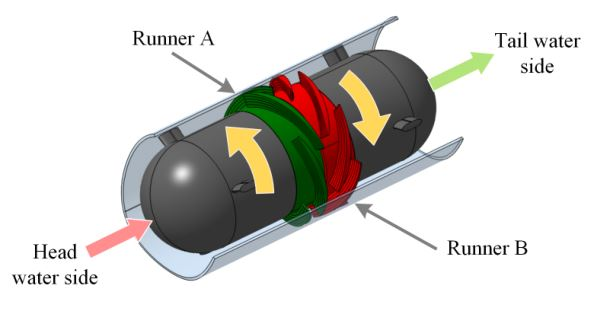
\includegraphics[scale=0.75]{counter_rotating_runners}
	\caption{Turbina contrarotativă \cite{andolfatto2016simulation}}
	\label{Turbina contrarotativă}
\end{figure}

\clearpage


\subsection{Utilizare modulară}
Unul din marile avantaje al acestor turbine axiale de destindere este posibilitatea de a le folosi modular în serie, forma lor compactă (vezi Figura 1.9) și cotele de gabarit reduse încurajând acest lucru.

\begin{figure}[h!]
	\centering
	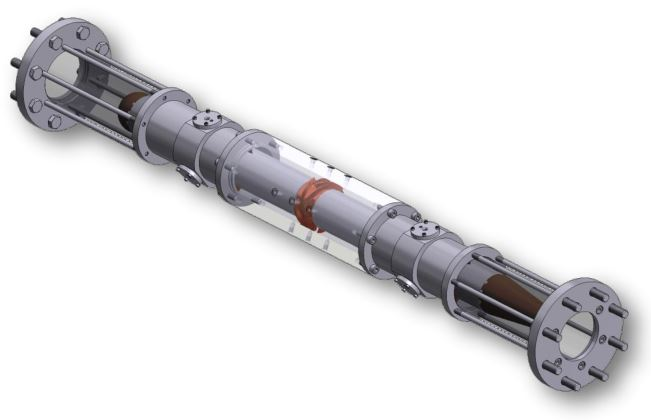
\includegraphics[scale=0.9]{modular}
	\caption{Posibilitate de montare modulară \cite{hasmatuchi2014new}}
	\label{Posibilitate de montare modulară}
\end{figure}

\subsection{Descrierea elementelor componente}

Principalele elemente componente ale turbinei axiale de destindere sunt:

\begin{itemize}
	\item \textbf{statorul}; conduce apa spre rotor și asigură vitezele respectiv circulația necesară transformării energetice optime, în condițiile pierderilor hidraulice minime.
	\item \textbf{rotorul}; are rolul de a transforma energia hidraulică disponibilă în energie cinetică, conducând apa care vine prin stator în tubul de aspirație al turbinei.
	\item \textbf{generatorul electric}; este un dispozitiv care transformă energia mecanică în energie electrică.
\end{itemize}


\section{Regimuri de funcționare}

Turbinele hidraulice se pot caracteriza din punct de vedere funcțional prin folosirea următorilor parametri:

\begin{itemize}
	\item debitul \textit{Q, $[\si{m}]$}
	\item căderea \textit{H, $[\si{m}]$}
	\item puterea \textit{$P_m$, $[\si{W}]$}
	\item viteza unghiular\u{a} \textit{\(\omega\), $[\si{rad/s}]$}
	\item randamentul \textit{\(\eta\), $[-]$}
	\item înălțimea geometrică de aspirație \textit{\(h_s\), $[\si{m}]$}
	\item coeficientul de cavitație \textit{\(\sigma\), $[-]$}
\end{itemize}


\subsubsection{Debitul}

Definim debitul volumic ca volumul de apă ce intră în turbină în unitatea de timp. Se exprimă în unități de volum, greutate sau de masă, raportate la unitatea de timp.


\subsubsection{Căderea turbinei}

Considerând secțiunea de la intrarea în turbină ca notată cu i și ieșirea cu e, căderea turbinei se exprimă sub forma $H=e_i-e_e$, deci

\begin{equation}
H=\bigg(\frac{p_i}{{\rho}g}+z_i+\frac{v_i^2}{2g}\bigg)_i-\bigg(\frac{p_e}{{\rho}g}+z_e+\frac{v_e^2}{2g}\bigg)_e \;[\si{m}]
\end{equation}

unde: $p\;[\si{Pa}]$ este presiunea, ${\rho}\;[\si{kg/m^3}]$ este densitatea apei, $z\;[\si{m}]$ este înălțimea, $v\;[\si{m/s}]$ este viteza iar $g\;[\si{m/s^2}]$ este accelerația gravitaționala.

\subsubsection{Puterea}

Puterea hidraulică sau puterea sursei $P_h$ este puterea disponibilă a apei de la intrarea în turbină pentru a putea fi transformată în putere mecanică la arborele turbinei:

\begin{equation}
P_h={\rho}gQH\; [\si{W}]
\end{equation}

Puterea mecanică a turbinei $P_m$ este puterea mecanică la arborele turbinei, obținută din momentul la arbore $M$ și viteza unghiulară $\omega$:

\begin{equation}
P_m=M{\omega}\; [\si{W}]
\end{equation}

\subsubsection{Turația}

Turația turbinei este numărul de rotații realizate în unitatea de timp, de obicei într-un minut (uneori în secundă). Se notează cu \textit{n} [rpm] sau cu \(\omega\) rad/s (SI).

\begin{equation}
n\; [\si{rpm}]\rightarrow{\omega}\; [\si{rad/s}]=\frac{{\pi}n}{30}
\end{equation}


\subsubsection{Randamentul}

În turbina hidraulică transmiterea energiei de la curentul de apă către rotor se efectuează cu pierderi. Acestea sunt definite și măsurate prin randamentul turbinei:

\begin{equation}
{\eta}=\frac{Putere\; utila}{Putere\; consumata}=\frac{P_m}{P_h}=\frac{M{\omega}}{{\rho}gQH}
\end{equation}


\subsubsection{Înălțimea geometrică de aspirație}

Înălțimea geometrică de aspirație este diferența în plan vertical dintre o referința a turbinei (de obicei planul care trece prin axa paletelor rotorului) și planul nivelului apei din aval.

\subsubsection{Coeficientul de cavitație}

Cavitația este un fenomen hidrodinamic complex, caracterizat de apariția, dezvoltarea și surparea rapidă a unor bule gravitaționale, umplute cu aburi și gaze, ce apare într-un curent de lichid în zona cu viteze mari și presiuni mici. Procesul fizic numit cavitație se apropie mai mult sau mai puțin de acela al fierberii lichidelor. Efectele principale ale cavitației sunt: vibrații si zgomote puternice, distrugerea materialului componentelor turbinei și scăderea randamentului de funcționare.

Aceste fenomene se intensifica atunci când pragul de cavitație limita este depășit, sau se funcționează în supercavitatie. Profesorul D.Thoma a introdus pentru prima oara noțiunea de prag de cavitație. Acest criteriu este denumit coeficient de cavitație și se exprima în felul următor:

\begin{equation}
\sigma=\frac{A-A\pm{H_s}}{H}
\end{equation}


\subsection{Valori tipice pentru parametrii fundamentali ai turbinelor de destindere}

În literatura de specialitate sunt investigate turbinele de destindere cu valori fundamentale care se încadrează deseori intre anumite limite.


\subsubsection{Debitul}
Pentru debitul volumetric valorile generale pe care le găsim în articolele științifice sunt următoarele:

\begin{itemize}
	\item 0.2500$\si{m^3/s}$ \cite{gentner2000experimentelle}
	\item 0.1200-0.1900$\si{m^3/s}$ \cite{GREES_2014}
	\item 0.0500-0.1450$\si{m^3/s}$ \cite{susanhub}
	\item 0.0090-0.0140$\si{m^3/s}$ \cite{biner2016engineering}
	\item 0.0375$\si{m^3/s}$ \cite{hasmatuchi2014new}
\end{itemize}

\subsubsection{Căderea}

\begin{itemize}
	\item 50$\si{m}$ \cite{gentner2000experimentelle}
	\item 40-200$\si{m}$ \cite{GREES_2014}
	\item 10.2-205.4$\si{m}$ \cite{susanhub}
	\item 24.265-61.162$\si{m}$ \cite{biner2016engineering}
	\item 29.9$\si{m}$ \cite{hasmatuchi2014new}
\end{itemize}


\subsubsection{Turația}

\begin{itemize}
	\item 1500$\si{rpm}$ \cite{gentner2000experimentelle}
	\item 3000$\si{rpm}$ \cite{GREES_2014}
	\item 1500 și 3000$\si{rpm}$ \cite{susanhub}
	\item 3000$\si{rpm}$ \cite{biner2016engineering}
	\item 3000$\si{rpm}$ \cite{hasmatuchi2014new}
\end{itemize}

Bazându-ne pe rezultatele din aceste studii putem concluziona ca domeniile de funcționare din Tabela 1.1 reprezinta un punct de plecare acceptabil pentru studiul care urmează.

\begin{table}[ht]
\caption{Domeniile de funcționare dorite ale turbinei AXENT \cite{neipp2017zweistufige}}% title of Table
\centering

\begin{tabular}{ c | c | c | c | c | c | c }
           & $Q_{min}$          & $Q_{max}$          & $H_{min}$    & $H_{max}$     & $n_{q,min}$        & $n_{q,max}$ \\ \hline
&&&&&&\\[-0.5em]
Valori țintă  & 0.05$\si{m^3/s}$ & 0.15$\si{m^3/s}$ & 10$\si{m}$ & 180$\si{m}$ & 15$\si{rpm}$ & 60$\si{rpm}$ \\
\end{tabular}

\end{table}


\subsection{Parametrii fundamentali aleși}

Conform lucrării de doctorat a lui Neipp \cite{neipp2017zweistufige} se pot îmbunătății caracteristicile de funcționare pentru o cădere $H$ mai mare mărind diametrul turbinei fata de turbina AXENT ($D_i = 0.14\si{m}$ și un diametru exterior $D_e = 0.18\si{m}$) dezvoltata inițial la Stuttgart. Astfel Neipp ajunge la un diametru exterior $D_e = 0.22\si{m}$. Pentru calculele viitoare folosim în continuare aceste valori pentru diametrul exterior, precum și debitul de $0.07\si{m^3/s}$, căderea este aleasa la valoarea de $H=24\si{m}$, iar turația este $n=1500\si{rpm}$.

\begin{table}[ht]
\caption{Parametrii fundamentali alesi}% title of Table
\centering

\begin{tabular}{ c | c | c | c }
$Q$ & $H$ & $n$ & $D_e$ \\ \hline
0.07$\si{m^3/s}$ & 24$\si{m}$ & 1500$\si{rpm}$ & 0.22$\si{m}$ \\
\end{tabular}

\end{table}

\clearpage